\section{Software-Entwicklung
\label{section:softwareengineering}}
In den folgenden Unterabschnitten wird die Architektur und Funktionsweise
des erarbeiteten Prototyps erklärt. Der Prototyp ist in Python geschrieben und
besteht aus fünf Klassen gemäss der Abbildung~\ref{figure:prototypearchitecture}.

\begin{figure}[h!]
	\centering
	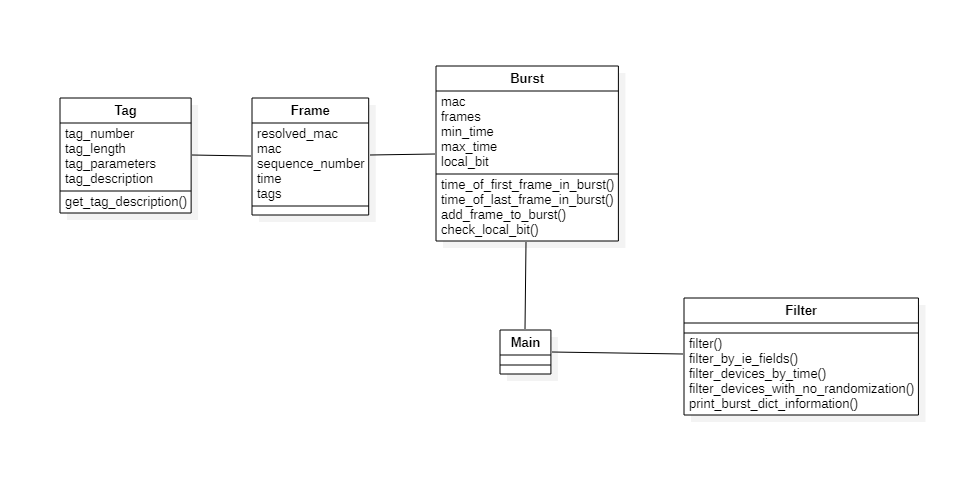
\includegraphics[width=1\linewidth]{Prototype/Klassendiagramm.PNG}
    \caption{Klassendiagramm des Prototyps
	\label{figure:prototypearchitecture}}
\end{figure}

\subsection{Beschreibung der Klassen}
\subsubsection*{Main-Klasse}
Die Main-Klasse ist der Einstiegspunkt in das Programm. 
Darin werden Probe-Requests aus einer angegebenem JSON-Datei ausgelesen,
decodiert und in Frame-Instanzen gespeichert. 
Diese Frame-Instanzen werden dann nach ihrer MAC-Adresse sortiert und 
in Burst-Instanzen gespeichert.
Nachdem die Probe-Requests durch das Preprocessing in Bursts gruppiert wurden,
wird eine Filterklasse instanziert und kann auf die Bursts angewandt werden.

\clearpage 

\subsubsection*{Burst-Klasse}
Ein Burst besteht aus mehreren Probe-Request-Frames mit der gleichen 
MAC-Adresse.
Die Burst Klasse beinhaltet einen bis mehrere Frames in einer Liste, 
welche aufsteigend nach der Ankunftszeit der Frames sortiert ist.
Die Tabelle~\ref{table:burstfields} beschreibt die Klassenvariablen.

\begin{table}[h!]
    \centering
    \begin{tabular}{|l|l|}
        \hline
        \textbf{Variable} & \textbf{Beschreibung} \\
        \hline 
        mac & Die MAC-Adresse der Frames im Burst. \\
        \hline
        frames & Eine Liste mit Frame-Objekten, die im Burst vorkommen. \\
        \hline
        min\_time & Ankunftszeit des ersten Frame im Burst. \\
        \hline
        max\_time & Ankunftszeit des letzten Frame im Burst. \\
        \hline
        local\_bit & Indikator, ob das lokale Bit gesetzt ist. \\
        \hline
    \end{tabular}
    \caption{Klassenvariablen der Burst-Klasse
    \label{table:burstfields}}  
\end{table}

Die Klasse beinhaltet vier Klassenmethoden gemäss der 
Tabelle~\ref{table:burstmethods}.

\begin{table}[h!]
    \centering
    \begin{tabular}{|l|l|}
        \hline
        \textbf{Methode} & \textbf{Beschreibung} \\
        \hline 
        time\_of\_first\_frame\_in\_burst & Evaluiert die Ankunftszeit des ersten \\
        & Frame im Burst. \\
        \hline
        time\_of\_last\_frame\_in\_burst & Evaluiert die Ankunftszeit des letzten \\
        & Frame im Burst. \\
        \hline
        add\_frame\_to\_burst & Fügt ein weiteres Frame zum Burst\\
        & hinzu. \\
        \hline
        check\_local\_bit & Evaluiert anhand der MAC-Adresse, \\
        & ob das local Bit gesetzt ist. \\
        \hline
    \end{tabular}
    \caption{Klassenmethoden der Burst-Klasse
    \label{table:burstmethods}}  
\end{table}

\clearpage 

\subsubsection*{Frame-Klasse}
Die Frame-Klasse beinhaltet jeweils einen einzelnen Probe-Request-Frame, 
welcher in den Messungen aufgezeichnet wurde.
Die Tabelle~\ref{table:framefields} beschreibt die Klassenvariablen. 
Die Frame-Klasse beinhaltet keine Klassenmethoden. 

\begin{table}[h!]
    \centering
    \begin{tabular}{|l|l|}
        \hline
        \textbf{Variable} & \textbf{Beschreibung} \\
        \hline 
        resolved\_mac & Die MAC-Adresse aufgelöst nach Hersteller, falls eine \\
        & Auflösung durch Wireshark vorgenommen wurde. \\
        \hline
        mac & Die MAC-Adresse des Frame. \\
        \hline
        sequence\_number & Die Sequenznummer des Frame. \\
        \hline
        time & Ankunftszeit des Frame. \\
        \hline
        tags & Liste mit Tag-Objekten, welche die \\ 
        & Information-Element-Felder 
        repräsentieren. \\
        \hline
    \end{tabular}
    \caption{Klassenvariablen der Frame-Klasse
    \label{table:framefields}}  
\end{table}

\subsubsection*{Tag-Klasse}
Tags werden verwendet, um die Information-Element-Felder zu repräsentieren.
Die verwendeten Klassenvariablen sind in der Tabelle~\ref{table:tagfields} 
dargestellt.

\begin{table}[h!]
    \centering
    \begin{tabular}{|l|l|}
        \hline
        \textbf{Variable} & \textbf{Beschreibung} \\
        \hline 
        tag\_number & Nummer des IE-Felds gemäss IEEE 802.11 \\
        \hline
        tag\_length & Grösse des Information-Element-Felds \\
        \hline
        tag\_parameters & Liste mit weiteren Informationen im IE-Feld. \\
        \hline
        tag\_description & Bezeichnung des Information-Element-Felds. \\
        \hline
    \end{tabular}
    \caption{Klassenvariablen der Tag-Klasse
    \label{table:tagfields}}  
\end{table}

Die Tag-Klasse beinhaltet die Klassenmethode "get\_tag\_description", 
welche aus einem Dictionary die Bezeichnung der Information-Element-Felder 
ausliest.

\clearpage

\subsubsection*{Filter-Klasse}
In der Filter-Klasse sind die einzelnen Filtermethoden umgesetzt, 
welche für die Klassifikation der Probe-Requests verwendet werden. 
Die Methoden nehmen als Input jeweils einen Dictionary mit Burst-Klassen 
entgegen und geben als Output ebenfalls einen Dictionary mit Burst-Klassen zurück.
Die Eigenschaft, dass der Input und Output der Methoden in identischem Format 
gehalten wird, erlaubt eine beliebige Reihenfolge der Methodenaufrufe.
Die einzelnen Filtermethoden sind in der Tabelle~\ref{table:filtermethods}
beschrieben.

\begin{table}[h!]
    \centering
    \begin{tabular}{|l|l|}
        \hline
        \textbf{Methode} & \textbf{Beschreibung} \\
        \hline 
        filter & Führt alle Filtermethoden \\
        & der Filterklasse aus. \\
        \hline
        filter\_by\_ie\_fields & Klassifiziert Frames anhand der \\
        & Information-Element-Felder. \\
        \hline
        filter\_devices\_by\_time & Klassifiziert Frames nach ihrer\\
        & Ankunftszeit. \\
        \hline
        filter\_devices\_with\_no\_randomization & Erkennt, ob in mehreren Bursts \\
        & die selbe MAC-Adresse verwendet\\ 
        &wurde  und fasst diese in einer\\
        & Liste zusammen. \\
        \hline
        print\_burst\_information & Methode für die Ausgabe der \\
        & Filterresultate. \\
        \hline
    \end{tabular}
    \caption{Klassenmethoden der Filter-Klasse
    \label{table:filtermethods}}  
\end{table}
       
Die Filterung nach Ankunftszeit kann, wie im 
Unterabschnitt~\ref{subsection:timefilter} beschrieben, 
nicht erfolgreich durchgeführt werden. 
Die Methode wurde der Vollständigkeit halber im Prototyp belassen, und kann 
verwendet werden, um aufzuzeigen, dass eine Filterung nach Ankunftszeit 
keine erfolgreiche Klassifikation durchführt.

\clearpage